\documentclass[]{beamer}
\mode<presentation>
{
  \usetheme{Warsaw}
  \definecolor{mcgarnet}{rgb}{0.38, 0, 0.08}
  \definecolor{mcgray}{rgb}{0.6, 0.6, 0.6}
  \setbeamercolor{structure}{fg=mcgarnet,bg=mcgray}
  %\setbeamercovered{transparent}
}


\usepackage[english]{babel}
\usepackage[latin1]{inputenc}
\usepackage{times}
\usepackage[T1]{fontenc}
\usepackage{tikz}
\usepackage{graphicx}

\newcommand{\imagesource}[1]{{\centering\hfill\break\hbox{\scriptsize Image Source:\thinspace{\small\itshape #1}}\par}}

\title{Object Oriented Programming -- Design}


\author{Dr. Robert Lowe\\}

\institute[Maryville College] % (optional, but mostly needed)
{
  Division of Mathematics and Computer Science\\
  Maryville College
}

\date[]{}
\subject{}

\pgfdeclareimage[height=0.5cm]{university-logo}{images/Maryville-College}
\logo{\pgfuseimage{university-logo}}



\AtBeginSection[]
{
  \begin{frame}<beamer>{Outline}
    \tableofcontents[currentsection]
  \end{frame}
}


\begin{document}

\begin{frame}
  \titlepage
\end{frame}

\begin{frame}{Outline}
  \tableofcontents
\end{frame}


% Structuring a talk is a difficult task and the following structure
% may not be suitable. Here are some rules that apply for this
% solution: 

% - Exactly two or three sections (other than the summary).
% - At *most* three subsections per section.
% - Talk about 30s to 2min per frame. So there should be between about
%   15 and 30 frames, all told.

% - A conference audience is likely to know very little of what you
%   are going to talk about. So *simplify*!
% - In a 20min talk, getting the main ideas across is hard
%   enough. Leave out details, even if it means being less precise than
%   you think necessary.
% - If you omit details that are vital to the proof/implementation,
%   just say so once. Everybody will be happy with that.

\section{Basic Concepts}
\begin{frame}{History \& Definitions}
    \begin{itemize}[<+(1)->]
        \item Developed slowly from the 1950s -- 1960s.
        \item Simula (1962) is largely regarded as the first true object
            oriented language. 
        \item OOP Rose to prominence in the 1980s -- 1990s with
            languages such as C++, Objective C, \& Java
        \item \textbf{Object Oriented Programming} -- A design
            paradigm where we decompose a problem into a set of
            objects which work together to solve a problem.
        \item \textbf{Object} -- An entity with state (attributes) and
            behavior (methods).
        \item \textbf{Class} -- A set of objects with the same
            attributes and methods.
    \end{itemize}
\end{frame}

\begin{frame}{Basic Principles of Object Oriented Programming}
    \begin{enumerate}[<+->]
        \item \textbf{Encapsulation/Data hiding} -- Access to attributes is
            controlled so objects maintain a valid state at all times.
        \item \textbf{Abstraction} -- Objects act as a ``black box'',
            and their use is separated from their implementation.
            (We neither know nor care how the object works!)
        \item \textbf{Inheritance} -- Classes can be related in
            a hierarchy of ``is-a'' relationships. For example: ``A
            squirrel is a mammal.''
        \item \textbf{Polymorphism} -- An object can simultaneously
            belong to multiple classes, yet still act as itself.  For
            example, if we know how to find the volume of a sphere, we
            can also find the volume of a basketball.
    \end{enumerate}
\end{frame}

\section{The Design Process}
\begin{frame}{Design Goals}
    \begin{enumerate}[<+->]
        \item \textbf{High Cohesion} -- Each object should have a well
            defined purpose for existing. No swiss army knives
            allowed!

        \item \textbf{Loose Coupling} -- Objects can use each other,
            but all code should depend upon only the public facing
            interface of an object.  Keep the internals of objects on
            a strict ``need to know'' basis.
    \end{enumerate}
\end{frame}

\begin{frame}{The Object Oriented Analysis and Design Process}
    \begin{enumerate}[<+->]
        \item Reason about the problem at hand, and identify objects
            from sample instances of the problem.
        \item Identify attributes within each object.
        \item Identify behaviors for each object.
        \item Group objects into classes based on their attributes and
            methods.
        \item List classes.
        \item Define class attributes.
        \item Define class methods \& constructors.
        \item Identify relationships among classes.
    \end{enumerate}
\end{frame}

\begin{frame}{UML -- Unified Modeling Language}
    \begin{itemize}[<+->]
        \item \textbf{UML} is a graphical design language which allows
            us to plan objects and classes in a programming 
            language-agnostic way.
        \item There are many UML diagrams; the most common being:
        \begin{itemize}
            \item Use Case Diagram
            \item Object Diagram
            \item Class Diagram
            \item Sequence Diagram
        \end{itemize}
        \item UML was developed by Rational Software from 1994-1996.
        \item UML became an ISO standard in 2005.
    \end{itemize}
\end{frame}

\begin{frame}{UML -- Object Diagram}
    \begin{columns}
    \column{0.5\textwidth}
    \begin{itemize}[<+->]
        \item An \textbf{Object Diagram} shows the state of various
            objects at some point in the program.
        \item Attributes and values are specified in the format:
            \newline \texttt{name = value}
        \item Names of objects are specified in the format:
            \newline \texttt{object : class}
        \item Lines between objects show that they are contained
            within each other.
    \end{itemize}

    \column{0.5\textwidth}
    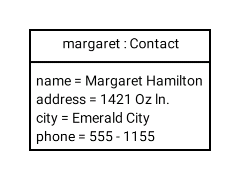
\includegraphics[width=\textwidth]{images/uml-object}
    \end{columns}
\end{frame}

\begin{frame}{UML -- Class Diagram}
    \begin{columns}
    \column{0.5\textwidth}
    \begin{itemize}[<+->]
        \item A class diagram shows classes and attributes.
        \item Attributes are listed in the format:
            \newline\texttt{name: type}
        \item Methods are listed as:
            \newline\texttt{name(p1:type, p2:type, $\ldots$) : type}
        \item Access modifiers are specified:
            \begin{itemize}
                \item \texttt{+} public
                \item \texttt{-} private
                \item \texttt{\#} protected
            \end{itemize}
    \end{itemize}
    \column{0.5\textwidth}
    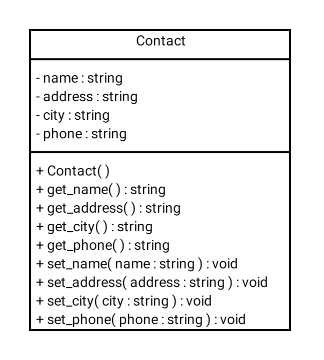
\includegraphics[width=\textwidth]{images/uml-class}
    \end{columns}
\end{frame}

\begin{frame}{Class Relationships -- Aggregation}
    \begin{itemize}[<+->]
        \item Aggregation is a basic ``has-a'' relationship.
        \item Objects of an aggregate class contain objects from
            another class.
        \item The objects are created and then given to the aggregate
            class.
        \item This is represented with an open diamond on the side of
            the aggregate.
            \newline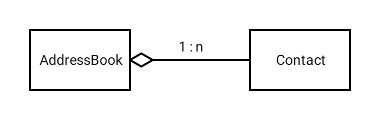
\includegraphics[height=2cm]{images/uml-aggregate}
    \end{itemize}
\end{frame}

\begin{frame}{Class Relationships -- Composition}
    \begin{itemize}[<+->]
        \item Composition is a stronger ``has-a'' relationship.
        \item Objects of a composite class contain objects from
            another class.
        \item The objects are created by the composite class.
        \item Composite objects fully own their parts.
        \item This is represented with a filled diamond on the side of
            the aggregate.
            \newline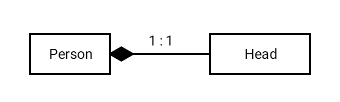
\includegraphics[height=2cm]{images/uml-composite}
    \end{itemize}
\end{frame}

\begin{frame}{An Intuitive Approach}
    \begin{enumerate}[<+->]
        \item Write out several scenarios for the use of your program.
            (This is a use case).
        \item Search for parts of speech:
            \begin{itemize}
                \item \textbf{Nouns} - Objects
                \item \textbf{Adjectives} - Attributes
                \item \textbf{Verbs} - Methods
            \end{itemize}
        \item Draw out objects.
        \item Look for container objects.
        \item Rework things until it is flexible enough.
        \item Design your classes from the new set of objects.
        \item Identify composition and aggregation relationships.
    \end{enumerate}
\end{frame}

\begin{frame}{Pattern: Accessors and Mutators}
    \begin{itemize}[<+->]
        \item One common design pattern is the use of accessors and
            mutators.
        \item Recall that all attributes should be private!
        \item An \textbf{accessors} is a function which returns the
            current value of an attribute.  
        \item A \textbf{mutator} is a function which sets the value of
            an attribute.
        \item Accessors are typically named \texttt{get\_<attribute>}.
        \item mutators are typically named \texttt{set\_<attribute>}.
        \item Why go to this level of trouble?
        \item This allows us to control/validate values and also make
            some attributes hidden and/or read only!
    \end{itemize}
\end{frame}

\begin{frame}{Class Activity: Design an Address Book}
    \begin{itemize}
        \item What sorts of thing do we want to do with an address
            book?
        \item What do the contact records look like?
        \item What do these things do with each other?
        \item Construct:
            \begin{itemize}
                \item Object Diagram
                \item Class Diagram
            \end{itemize}
        \item What relationships exist between the classes?
    \end{itemize}
\end{frame}

\section{Designing the Stock Program}

\begin{frame}{The Stock Program (Program 5)}
    \begin{itemize}
        \item Play with the stock program solution and read the
            program specification.
        \item Draw an object diagram.
        \item Draw a class diagram.
        \item Identify relationships.
    \end{itemize}
\end{frame}

\end{document}


